\documentclass[a4paper, 11pt, titlepage]{article}
\setlength{\oddsidemargin}{0in} \setlength{\evensidemargin}{0in}
\setlength{\textwidth}{6.2in}
\setlength{\topmargin}{-0.2in} \setlength{\textheight}{8.8in}

\usepackage{graphicx}
\graphicspath{ {/home/michal/development/workspace/CS12320_assign2/doc/img/} }

\title{Individual Assignment: Patience is a Virtue}
\author{Michal Wojciech Goly [mwg2]}
\date{1st May 2015}

\begin{document}

\maketitle
\tableofcontents
\newpage

\section{Introduction}
\subsection{Project description}
Patience is a simple card game for one player, in which the objective is to end up with 
one pile of cards on the table. There are 52 playing cards at the start of the game, all
facing downwards in a pack. Player can then deal a card which will be removed from the
deck and put on the table facing upwards. By continuing to do so, there could potentially
be 52 cards on the table all facing upwards, unless a different move was made. Apart from
dealing cards there are two additional valid moves in the game. Cards can be joined 
together if they have the same suit or value and if:
\begin{itemize}
	\item They are next to each other
	\item There are two other cards between them
\end{itemize}
When joined, the card further to the right will be placed on top of the other, regardless
of the order in which they have been selected. Each move is worth 10 points in the game. 
Therefore because there are 51 available moves in total, the highest possible score is
510 points. 

\subsection{Game controls} 
Because the user interface is fully graphical, to play the game user can simply click on 
the cards. For example if the player wants to deal a card, he should click on the pack 
and a move will be made. Similarly, to select a card user has to click on it. In order to
indicate which card was selected, a blue border will be painted around it.

Additional options are available within the button panel at the bottom of the window. 
Player can display contents of the pack, as well as shuffle it. Second option is only
permitted once and should typically be selected at the start of the game. Pack is not 
randomized by default due to the requirements specification of the assignment. Last two
options allow an automation of the gameplay. Player can either make use of the 'Play for
me once' option which as expected will make one valid move in the game, if there is one,
or specify the amount of moves to be made by clicking the 'Play for me x times' button.

Game ends either if the automation algorithm detects that there are no more moves 
available, user presses the 'x' exit button on the top of the window or game is won.
Before the application closes, a smaller window will pop up to ask the player to enter
his name in order to save his score. User can choose not to store his result by leaving
the name field blank.

\newpage

\section{Requirements Analysis}
\subsection{UML Use Case diagram}
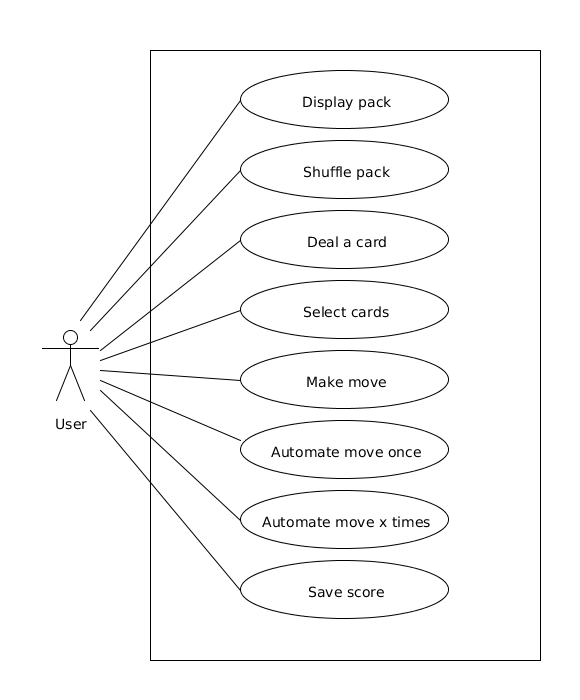
\includegraphics[width=\textwidth]{useDiagram}

\section{Design}
\subsection{UML Class diagram}
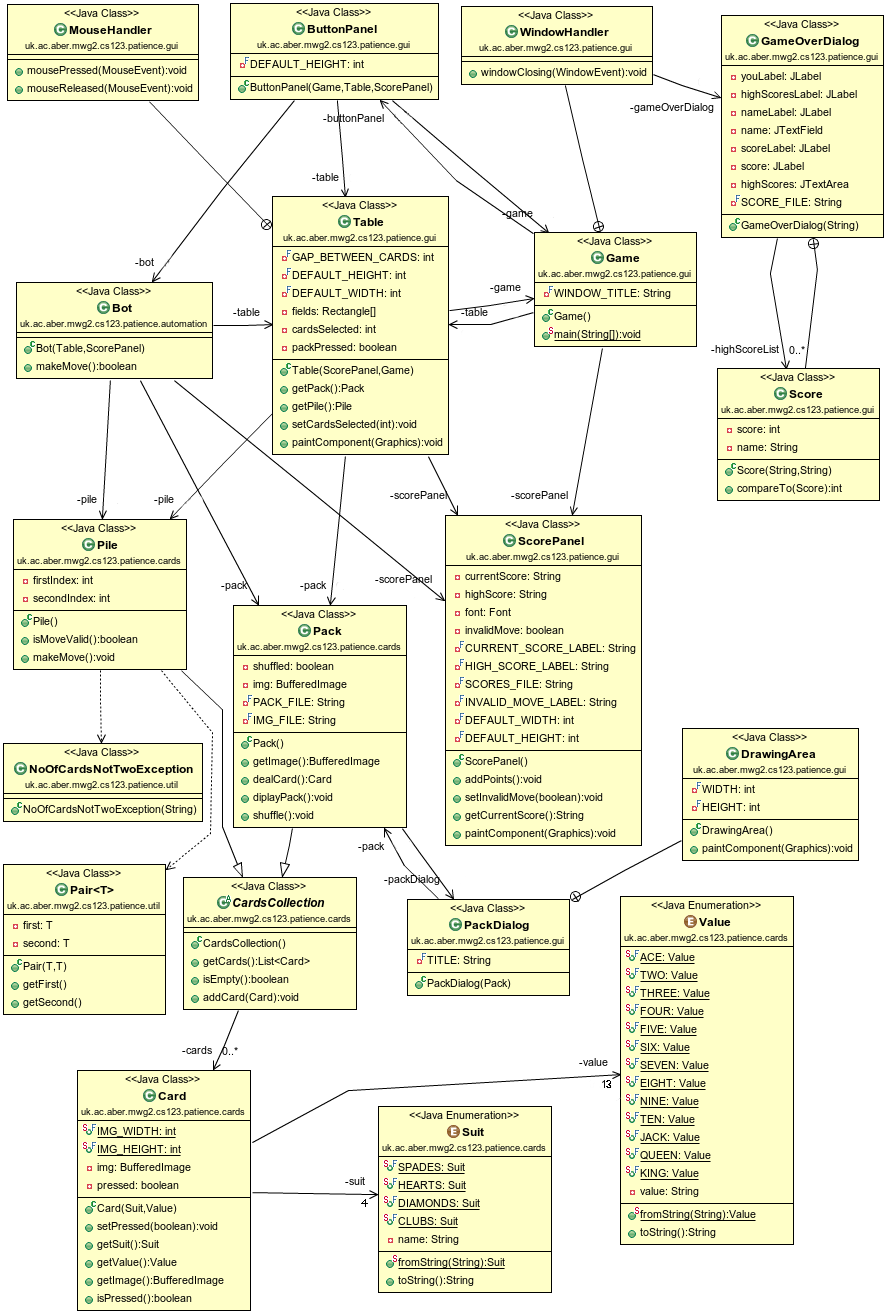
\includegraphics[width=\textwidth]{classDiagram}

\subsection{Description and relationships of each Class}
\begin{enumerate}
	\item \texttt{Game} class contains the \texttt{main} method and is therefore the 
		starting point of the application. It also extends the \texttt{JFrame} class and 
		takes care of the initialzation and layout of the \texttt{ScorePanel}, 
		\texttt{Table} and \texttt{ButtonPanel} components within itself.
		
	\item \texttt{WindowHandler} is an inner class implemented inside the \texttt{Game}
		class. It extends the \texttt{WindowAdapter} class, which means that it can 
		listen and react to the events generated by the window. Whenever a window closing 
		event is being dispatched, this class displays a \texttt{GameOverDialog} dialog.
		
	\item \texttt{GameOverDialog} is displayed whenever user wins the game or decides to
		exit the window. He will be then asked to enter his name which will be saved
		alongside his score. Previously recorded scores are stored inside a txt file
		\texttt{scores.txt} and are loaded into a list of objects of type \texttt{Score}
		whenever game is launched.
		
	\item \texttt{Score} is an inner class located inside the \texttt{GameOverDialog}. 
		It holds an information about the name of the player, his score and enables the
		list of scores to be sorted in a descending order. 
		
	\item \texttt{ScorePanel} is a GUI \texttt{JPanel} on top of the window. It displays
		the current score of the player, as well as the highest score recorded in the 
		past. Object of this class can be notified if an invalid move has been detected 
		in the game, via the \texttt{setInvalidMove} method. Appropriate message will be 
		displayed to notity the player about it. Similarly, other objects can call 
		the \texttt{addPoints} method to add 10 points to the current score and update
		the view.
		
	\item \texttt{Table} extends the \texttt{JPanel} class and represents the playing 
		table on which cards are being printed. \texttt{Pile} is printed on the top of 
		the panel, while \texttt{Pack} on the bottom. \texttt{Table} object acts the 
		view, whereas its inner class \texttt{MouseHandler} as the controller. 
		It will update itself whenever it is notified about the change of
		either the \texttt{Pack} or the \texttt{Pile} contents. Furthermore, a blue border
		will be painted around each selected card in the game.
		
	\item \texttt{MouseHandler} extends the \texttt{MouseAdapter} class and reacts to
		the events generated by player's mouse. It acts as the controller and enables the 
		user to manipulate cards by clicking and selecting them. Whenever a card is 
		selected, \texttt{MouseHandler} will notify the view \texttt{Table} to update 
		itself. \texttt{MouseHandler} is also making sure that the maximum number of 
		cards selected at any time is not greater than 2. If user selects two cards, 
		\texttt{MouseHandler} will try to make a move by calling the \texttt{isMoveValid}
		 and \texttt{makeMove} methods from the \texttt{Pile} object. Then it will 
		 tell the \texttt{ScorePanel} to either add 10 points to the current score or
		 display the "INVALID MOVE" notification. Finally, it will dispach the window 
		 closing event in case the user wins the game.
		 \begin{enumerate}
			 \item \texttt{Detect mouse pressed event\\
				Clear the 'invalid move' notification from the panel\\
				Check if any of the cards contain coordinates of the event\\
				If so, select this card\\
				Ask table to update itself
				}
			\item \texttt{Detect mouse released event\\
				If two cards are selected, make a move or unselect if its illegal\\
				Ask table to update itself\\
				Check if player won and finish the game if he did
				}
		\end{enumerate} 
		
	\item \texttt{ButtonPanel} is located on the bottom of the window and contains
		buttons user can click to access additional functions. Displaying
		\& shuffling the pack and automation of the gameplay. 
		
	\item \texttt{CardsCollection} is an abstract class which represents a collection of 
		cards. Internally cards are stored in a list and can be accessed and removed 
		using provided methods.
		
	\item \texttt{Pack} extends the \texttt{CardsCollection} and represents a 52 cards 
		pack. Cards can be shuffled once and removed from the pack using the 
		\texttt{shuffle} and \texttt{dealCard} methods respectively. If the 
		\texttt{displayPack} method is called, a dialog will pop up showing the contents 
		of the \texttt{Pack}.
	
	\item \texttt{PackDialog} is a modal dialog box which consists of two components. 
		In the centre of the box, a \texttt{DrawingArea} paints current contents of the
		\texttt{Pack}. A button panel is situated on the bottom of the window enabling
		the player to close the dialog.  
	
	\item \texttt{DrawingArea} is an inner class inside the \texttt{PackDialog}, which 
		extends the \texttt{JPanel} and overrides the \texttt{paintComponent} method. Its
		only purpose is to graphically display contents of the \texttt{Pack}.		
	
	\item \texttt{Pile} extends the \texttt{CardsCollection} and represents cards 
		dealt from the \texttt{Pack} on to the \texttt{Table}. It also holds the 
		information about the indexes of the cards which are currently selected. It has 
		two very important methods \texttt{isMoveValid} and \texttt{makeMove}. First one 
		checks if the two selected cards correspont to any of the known moves in the 
		game, while the second one actually makes the move. \texttt{isMoveValid} has to 
		be called before the other one. 

	\item \texttt{NoOfCardsNotTwoException} is thrown whenever the number of pressed 
		cards is not as expected equal to 2. 
	
	\item \texttt{Pair<T>} a simple generic class which represents a pair of any two 
		objects of the same class. Allows to easily pass around two objects together.

	\item \texttt{Card} class represents a single playing card. Each card has its value, 
		suit and an image. An appropriate picture is loaded depending on the suit and
		the value of the card. 
	
	\item \texttt{Suit} enum represents a suit of a card. Each suit has its corresponding
		single character String representation, accessible with the \texttt{toString} 
		method.
	
	\item \texttt{Value} enum represents a value of a card. Each value has its String 
		representation, accessible with the \texttt{toString} method.

	\item \texttt{Bot} object can be used to automate the game. Its only public method
		\texttt{makeMove} tries to make a move in the game and returns \texttt{true} if
		it succeeds or \texttt{false} otherwise. Cards in the \texttt{Pile} are firstly 
		checked from right to left to see whether it is possible to join any (make a 
		move). If none of the cards can be combined, bot will try to deal a card from 
		the \texttt{Pack}. If that fails then the game is over as there are no more
		available moves, and an appropriate event will be dispatched to display the
		\texttt{GameOverDialog}.
		
		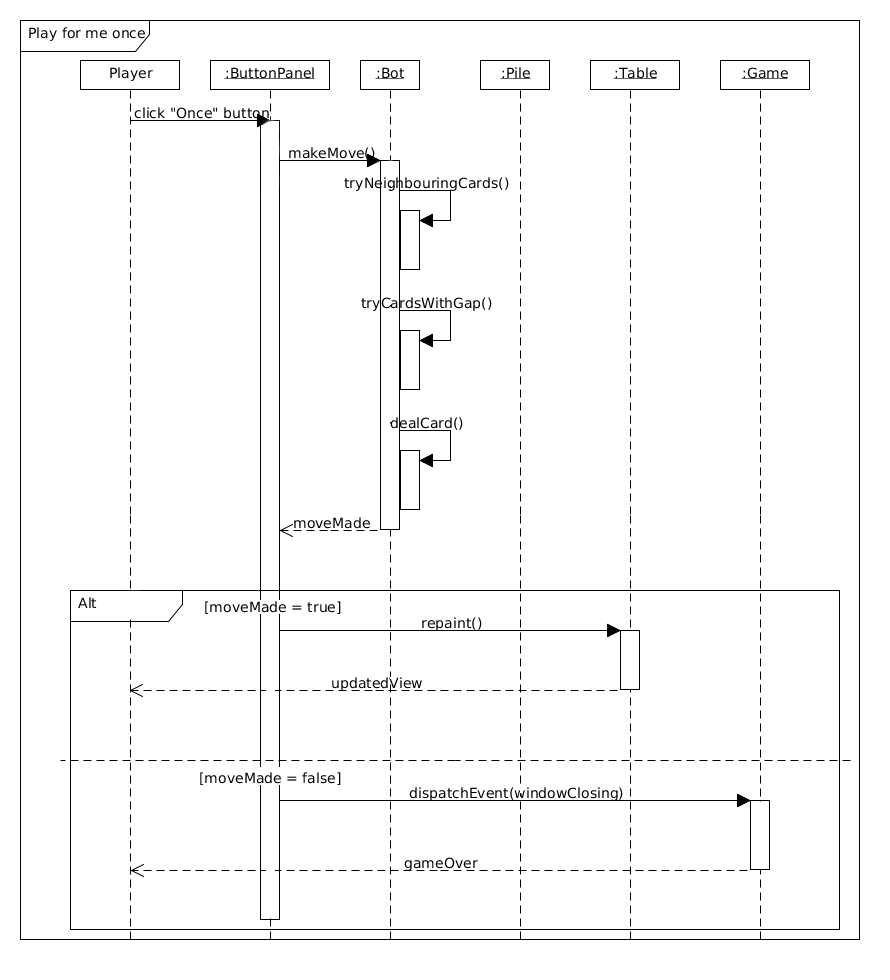
\includegraphics[width=\textwidth]{sequence}
	
\end{enumerate}

\section{Testing}
\subsection{Test tables}
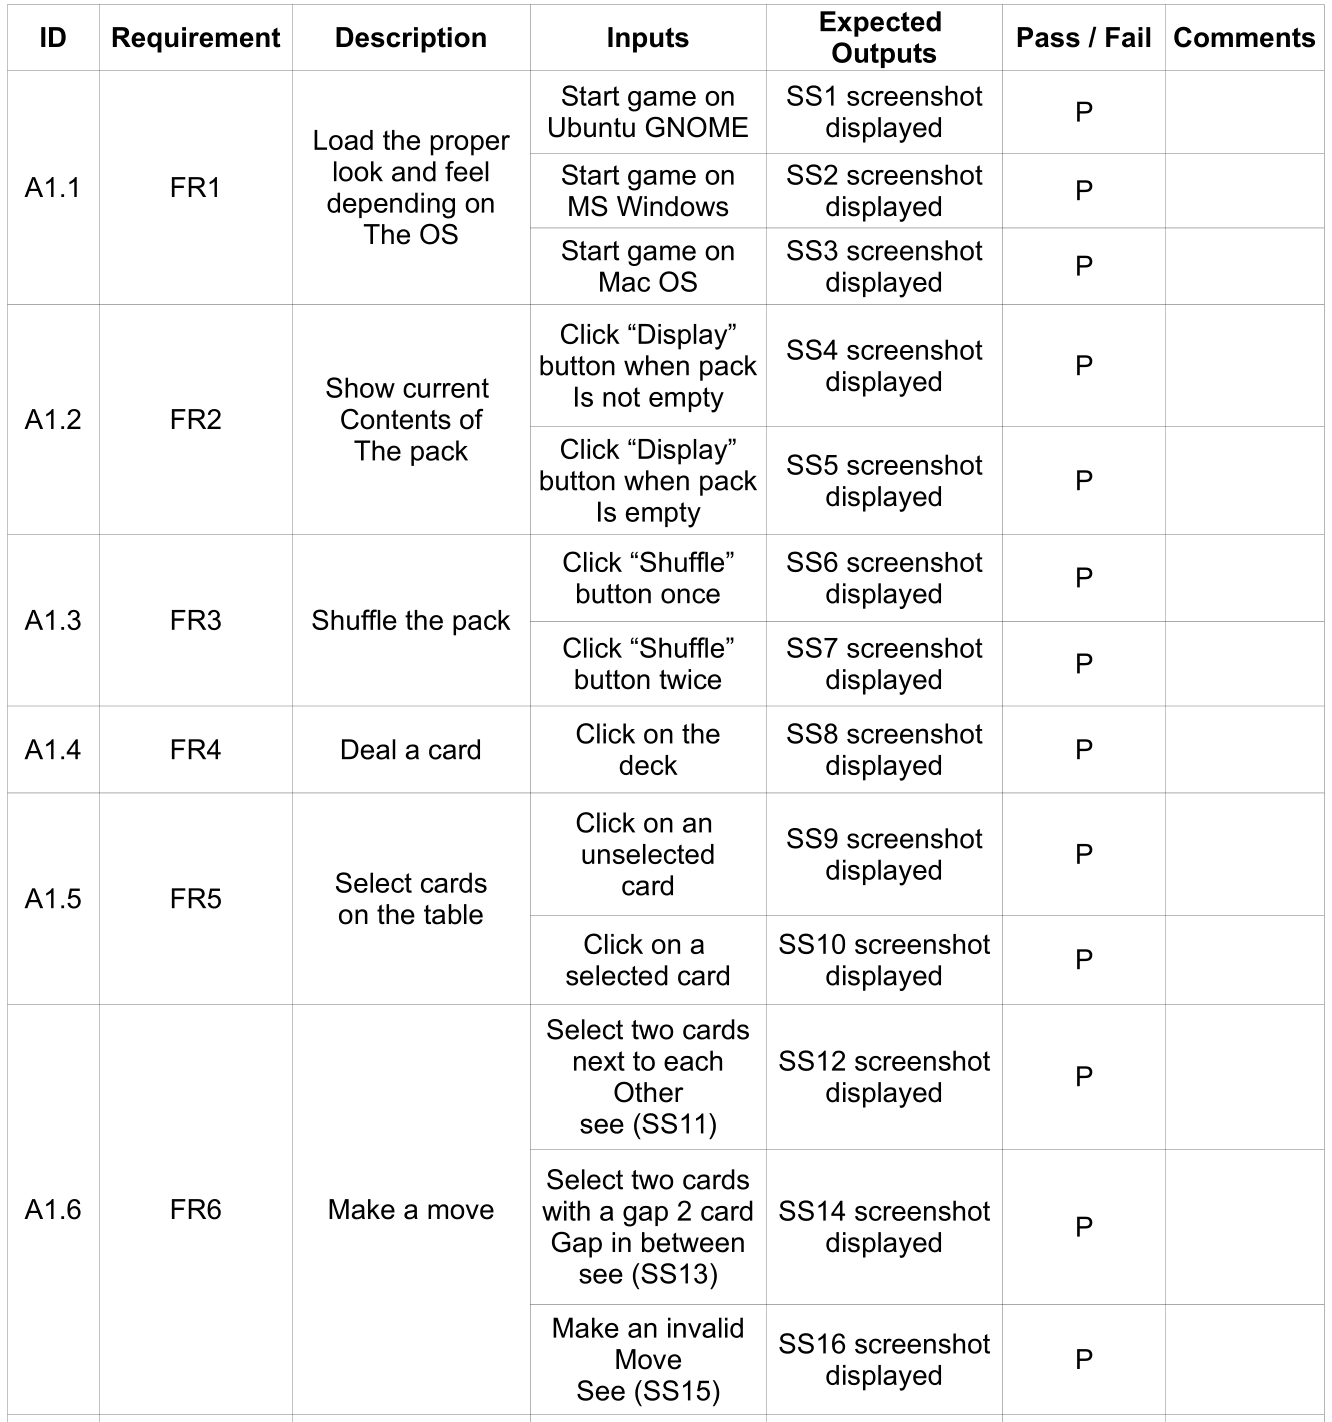
\includegraphics[width=\textwidth]{tableA}
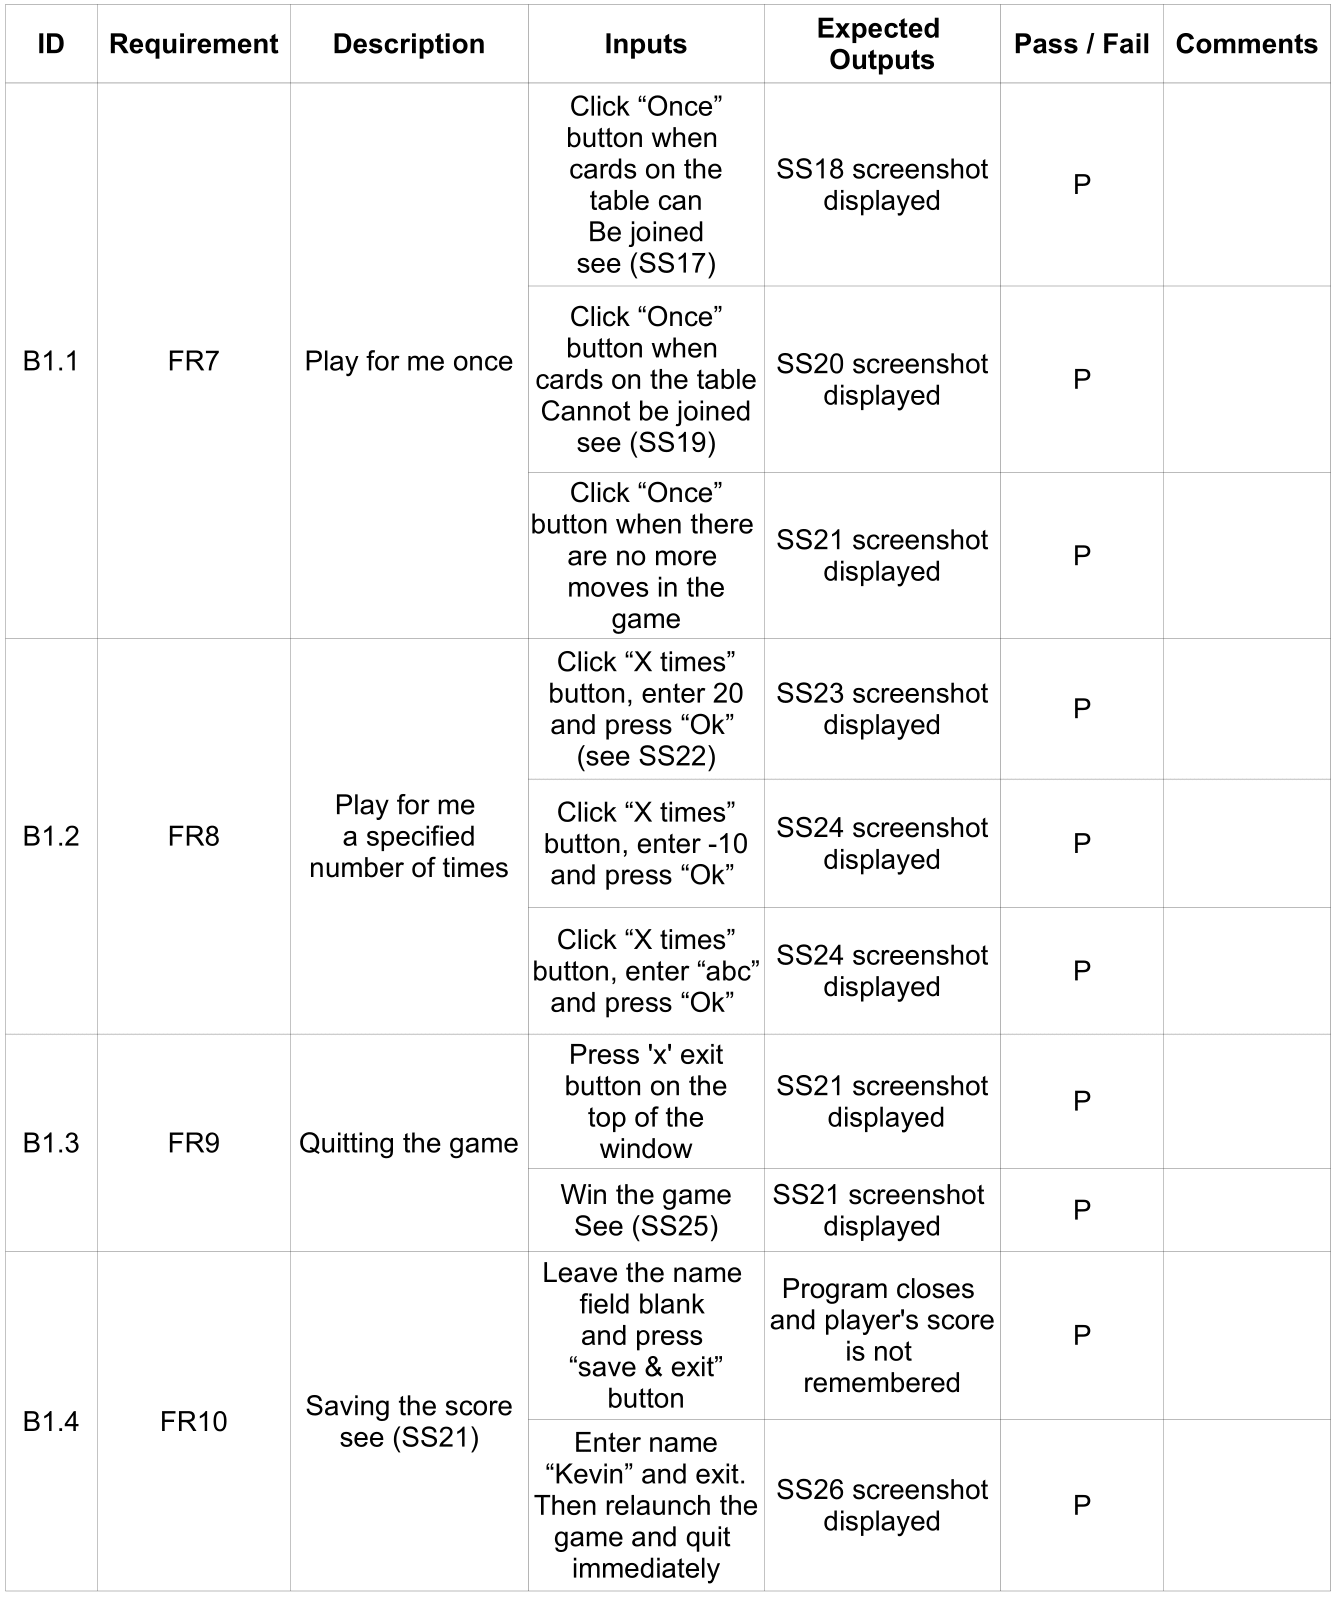
\includegraphics[width=\textwidth]{tableB}
\newpage

\subsection{Screenshots}
\begin{enumerate}
	\item[SS]1\\\\
		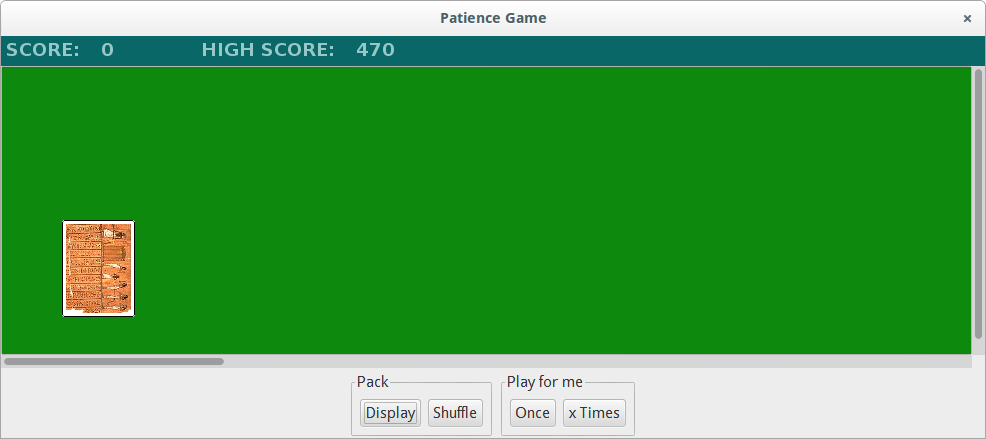
\includegraphics[width=\textwidth]{ss1}
	\item[SS]2\\\\
		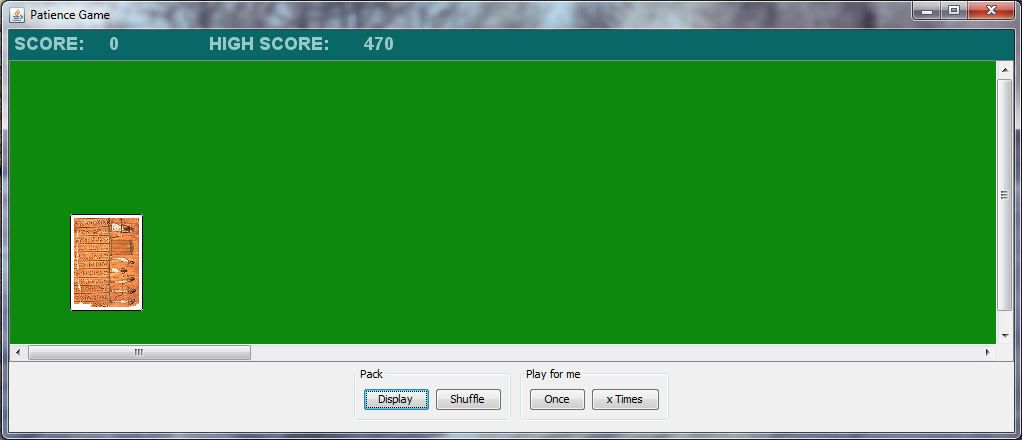
\includegraphics[width=\textwidth]{ss2} \newpage
	\item[SS]3\\\\
		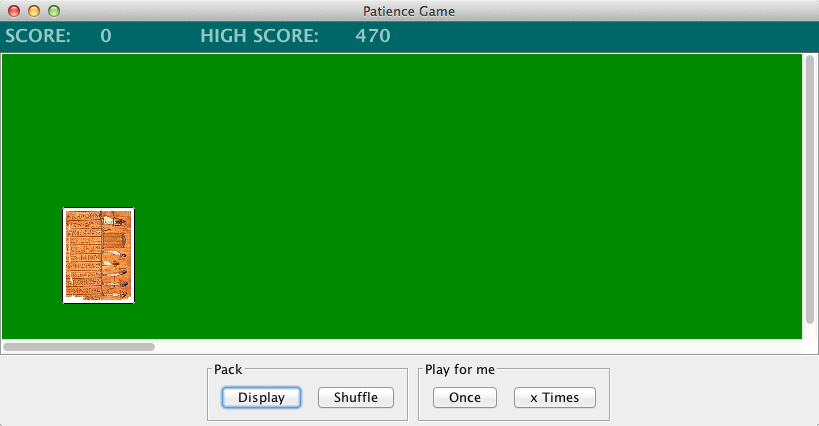
\includegraphics[width=\textwidth]{ss3}
	\item[SS]4\\\\ 
		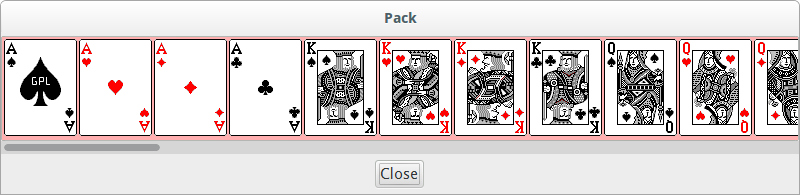
\includegraphics[width=\textwidth]{ss4}
	\item[SS]5\\\\ 
		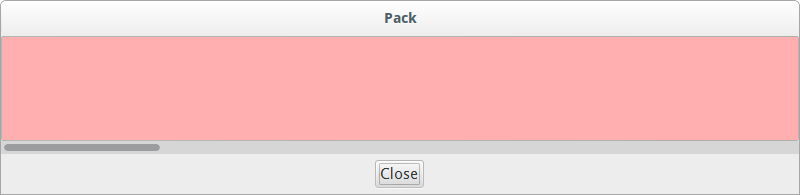
\includegraphics[width=\textwidth]{ss5} \newpage
	\item[SS]6\\\\
		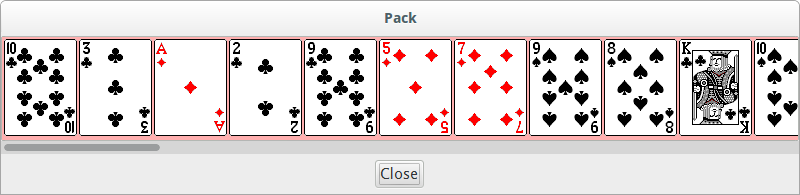
\includegraphics[width=\textwidth]{ss6}
	\item[SS]7\\\\ 
		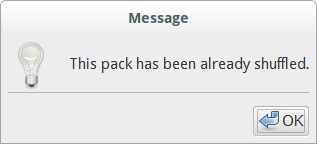
\includegraphics[width=0.4\textwidth]{ss7}
	\item[SS]8\\\\ 
		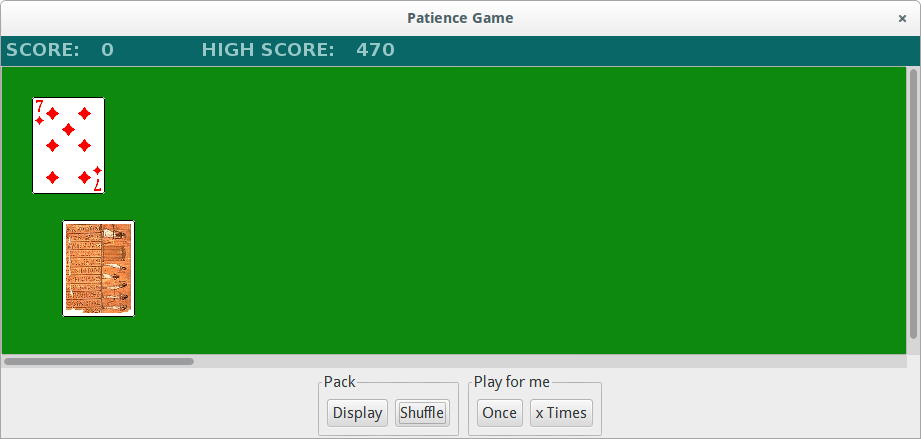
\includegraphics[width=\textwidth]{ss8} \newpage
	\item[SS]9\\\\ 
		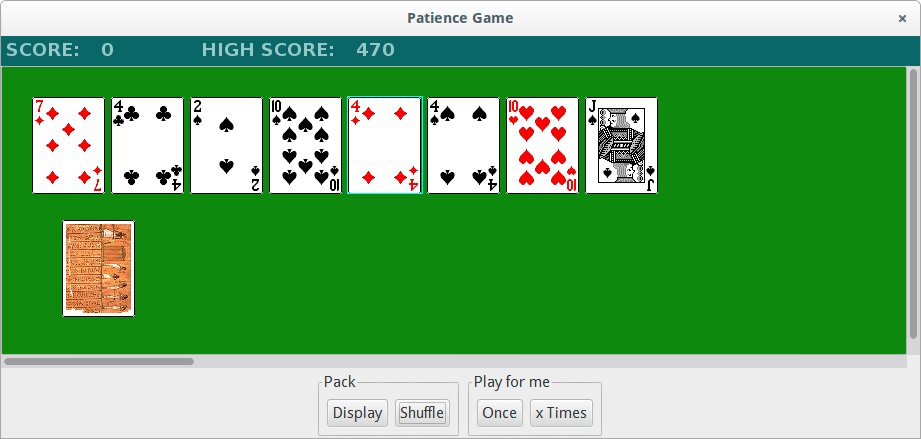
\includegraphics[width=\textwidth]{ss9}
	\item[SS]10\\\\ 
		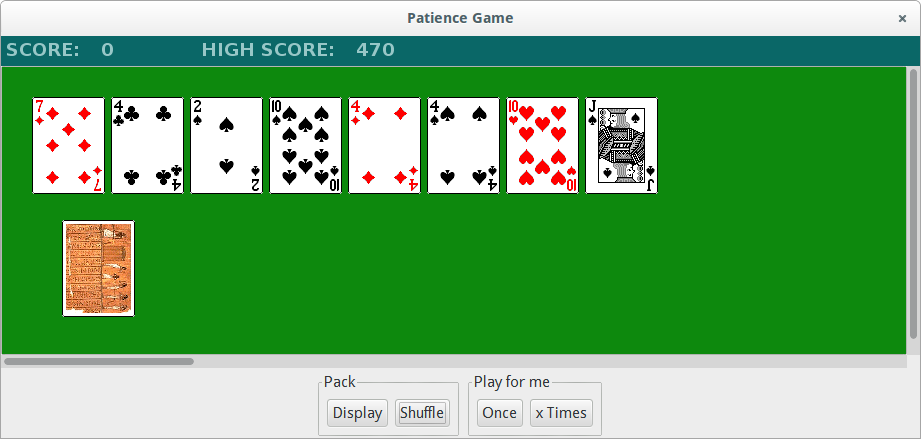
\includegraphics[width=\textwidth]{ss10} \newpage
	\item[SS]11\\\\ 
		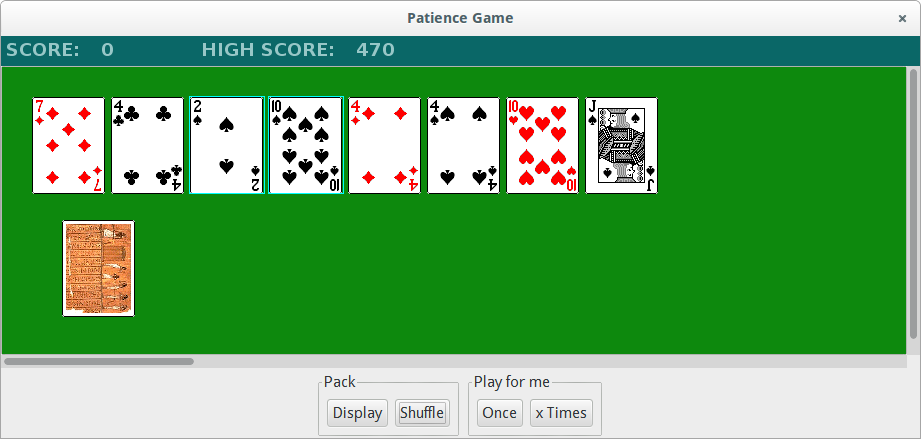
\includegraphics[width=\textwidth]{ss11}
	\item[SS]12\\\\ 
		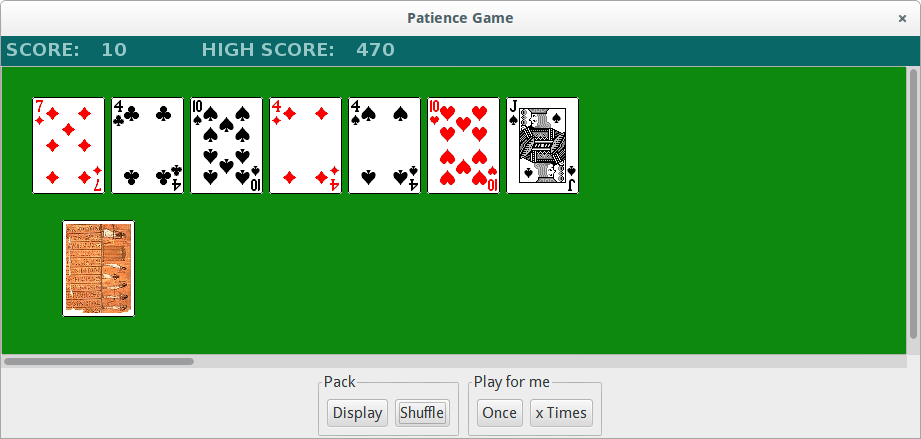
\includegraphics[width=\textwidth]{ss12} \newpage
	\item[SS]13\\\\ 
		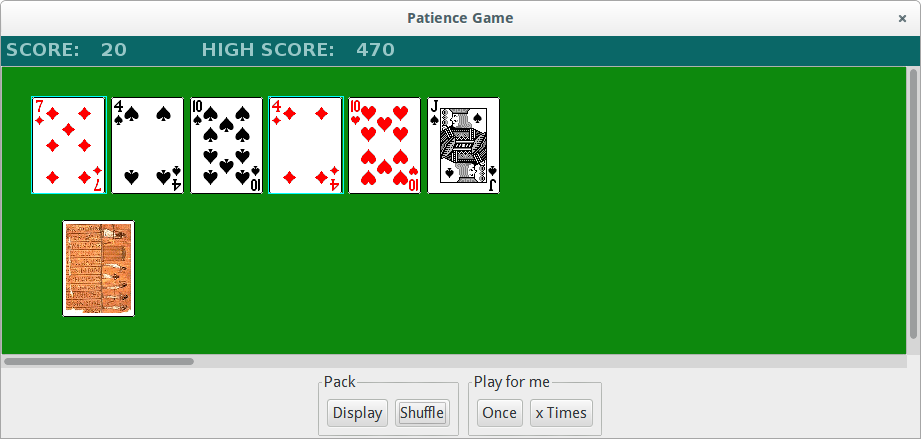
\includegraphics[width=\textwidth]{ss13}
	\item[SS]14\\\\ 
		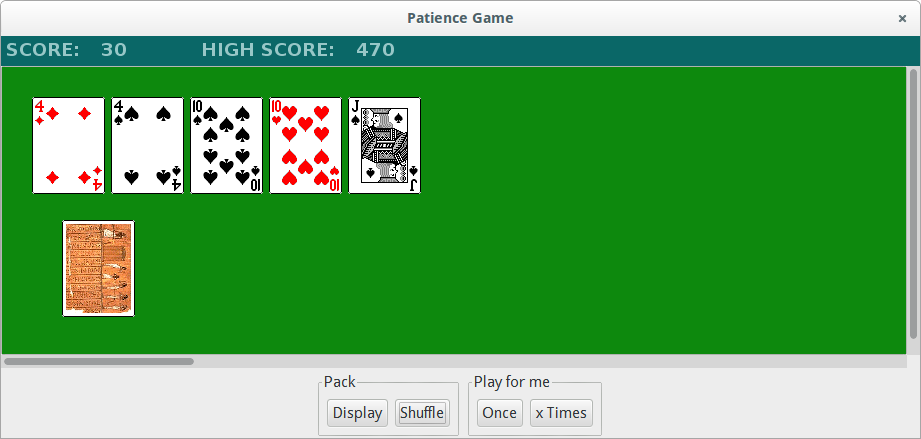
\includegraphics[width=\textwidth]{ss14} \newpage
	\item[SS]15\\\\ 
		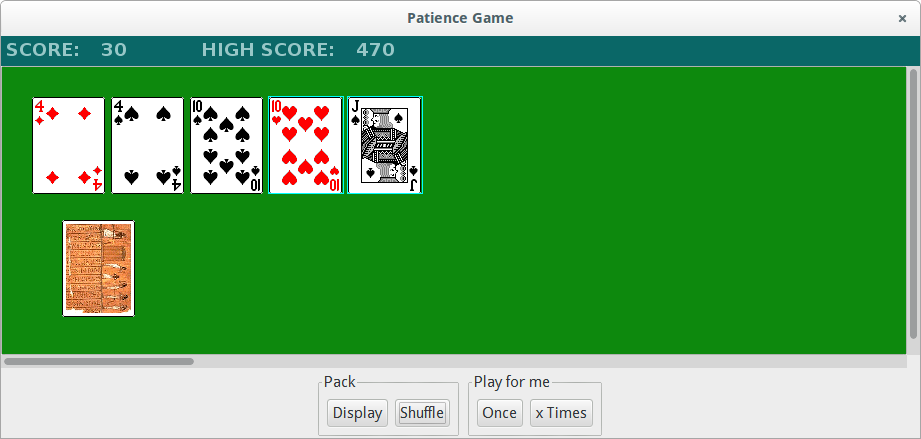
\includegraphics[width=\textwidth]{ss15}
	\item[SS]16\\\\ 
		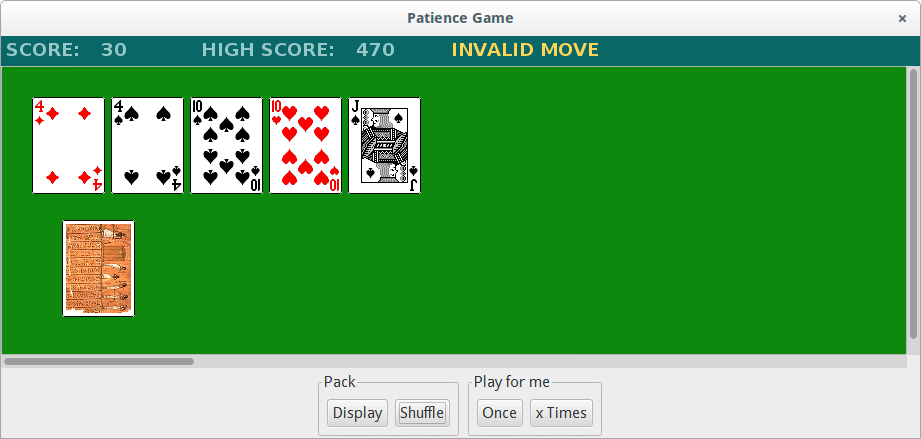
\includegraphics[width=\textwidth]{ss16} \newpage
	\item[SS]17\\\\ 
		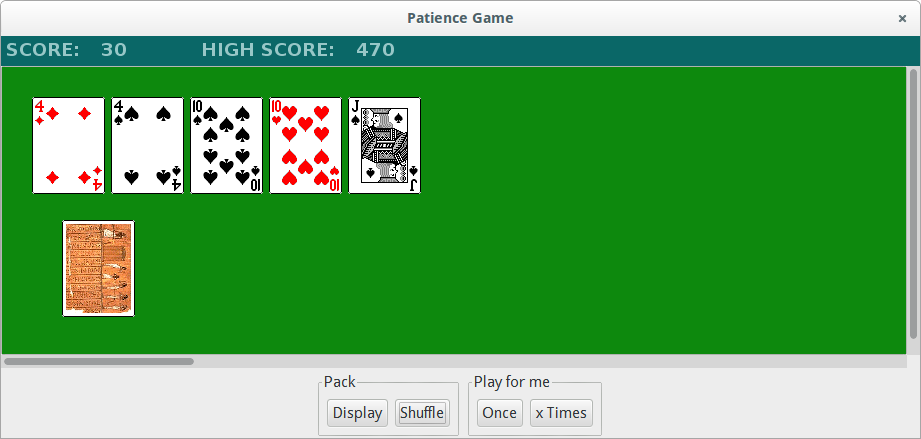
\includegraphics[width=\textwidth]{ss17}
	\item[SS]18\\\\ 
		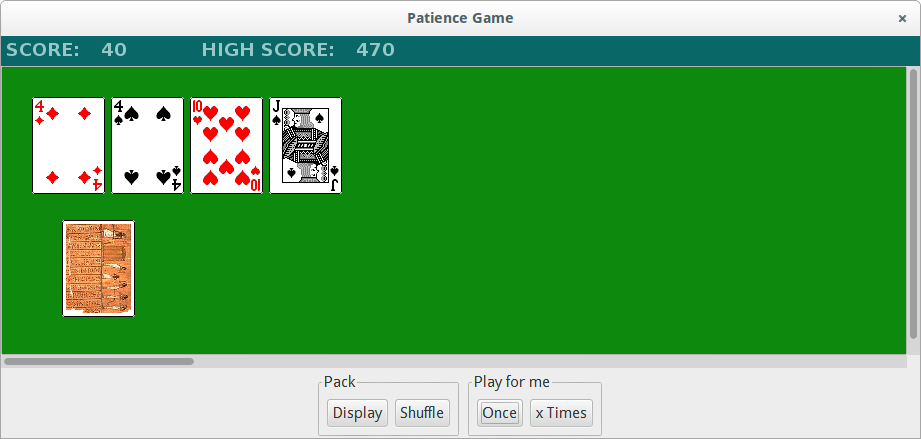
\includegraphics[width=\textwidth]{ss18} \newpage
	\item[SS]19\\\\ 
		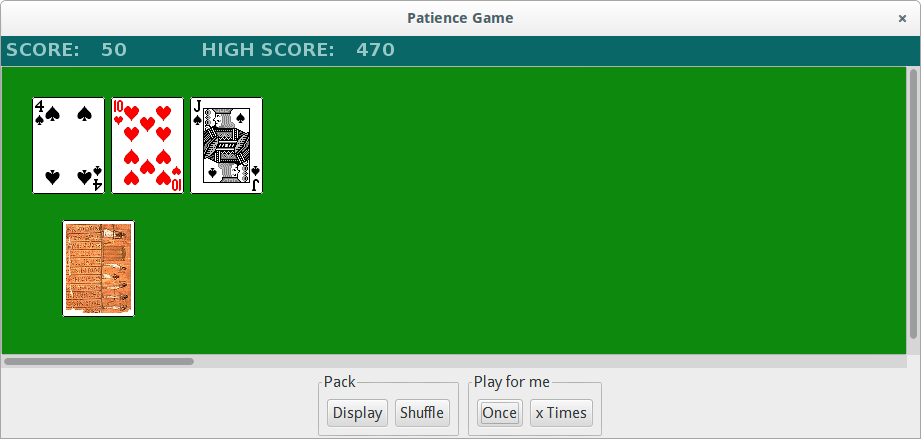
\includegraphics[width=\textwidth]{ss19}
	\item[SS]20\\\\ 
		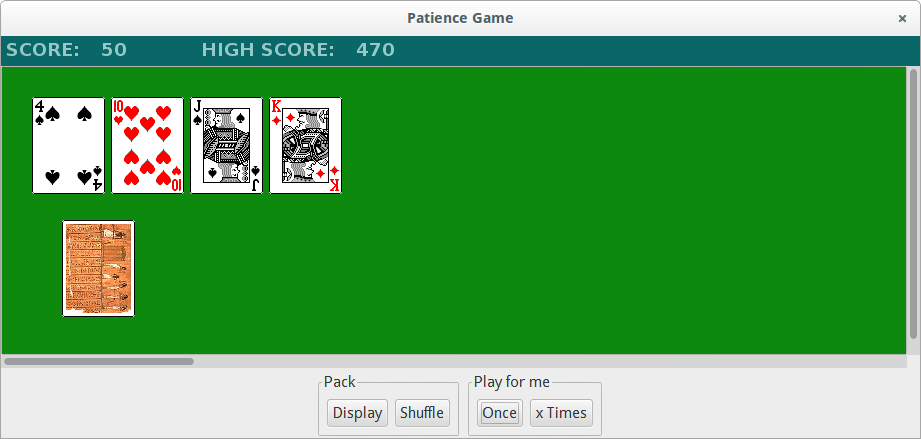
\includegraphics[width=\textwidth]{ss20} \newpage
	\item[SS]21\\\\ 
		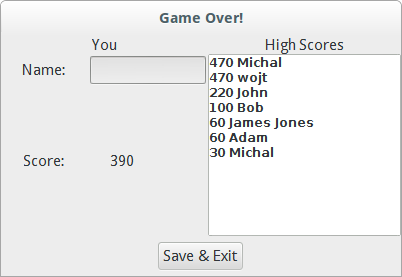
\includegraphics[width=0.6\textwidth]{ss21}
	\item[SS]22\\\\ 
		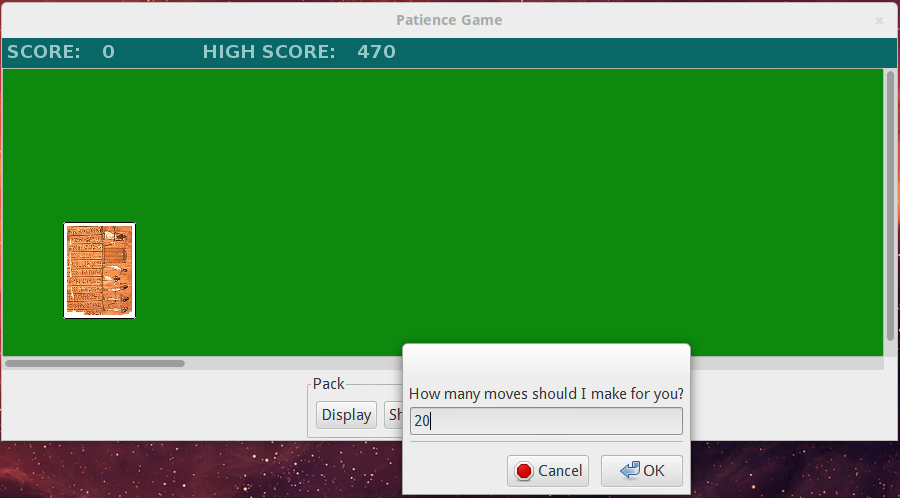
\includegraphics[width=\textwidth]{ss22} \newpage
	\item[SS]23\\\\ 
		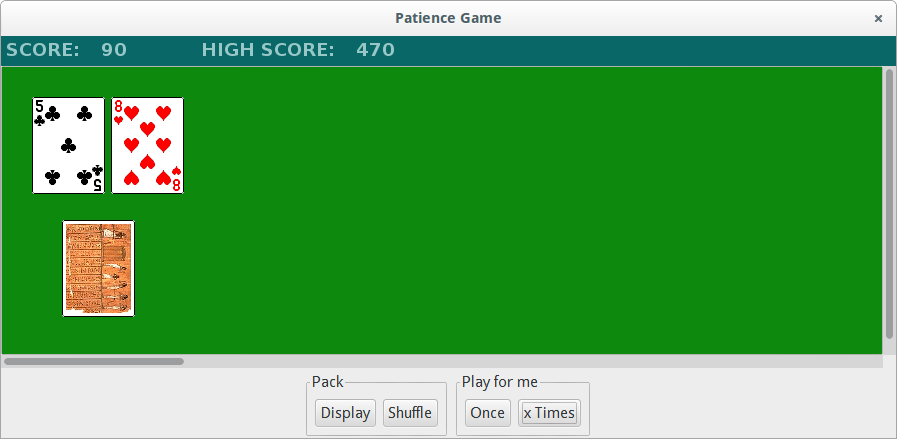
\includegraphics[width=\textwidth]{ss23}
	\item[SS]24\\\\ 
		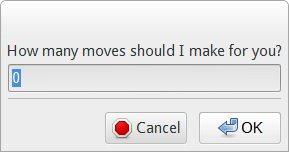
\includegraphics[width=0.4\textwidth]{ss24} \newpage
	\item[SS]25\\\\ 
		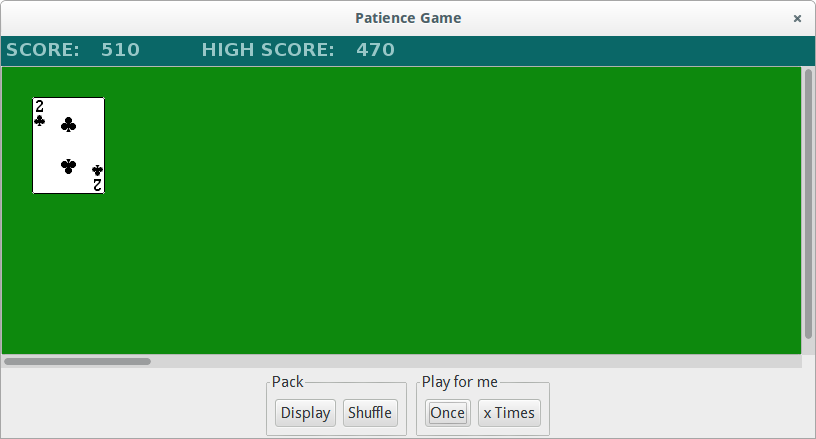
\includegraphics[width=\textwidth]{ss25}
	\item[SS]26\\\\ 
		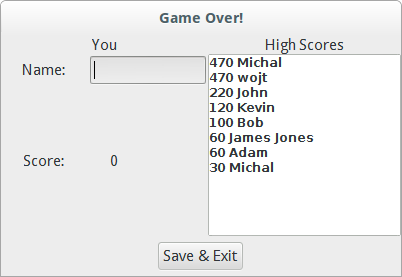
\includegraphics[width=0.6\textwidth]{ss26}		
\end{enumerate}
\section{Evaluation}
I began by reading the requirements specification and trying to understand the rules
of the game. Unlike in the previous mini-assignments, we did not receive an initial 
implementiation of the program. Therefore I realised that I should not rush into 
writing the code, before creating a simple design of the system. At this point I knew,
that I am going to need to represent playing cards, their suits and values, pack and 
some sort of collection of cards the player could select. 

\subsection{Completely graphical user interface}
I have been asked to create a console application which could also take the advantage of 
the GUI framework provided. Player could then type in commands from the menu and 
make moves in the game. The GUI frame would be used to graphically display his progress. 

In order to make the assignment more challenging and fun, I have decided to make the 
application completely graphical. User could then click on cards and buttons rather than
typing commands into console. This approach however, eliminated the point of the two 
requirements in the specification of the assignment. Without the console, "control text
display" option could not be implemented, nor could be printing of the output into a 
text file. Furthermore, the "display pack" option could not just print deck's contents.
Instead it displays a modal dialog box which graphically presents cards in the pack.

\subsection{Initial implementation}
\texttt{Card} was the first class I wrote and straight away I knew that apart from 
keeping the track of its suit and value, it would also need to know whether it has been
pressed or not. A boolean instance variable was a sufficient solution to that problem. 
Subsequently, I moved on to create a \texttt{Pack} which would initialy store 52 ordered
playing cards. \texttt{Pile} class represents the cards which were delt from the pack
on to the table. Because it has similar basic behaviour as the \texttt{Pack}, I have
decided to use inheritance and abstract this functionality into a parent class called
\texttt{CardsCollection}. 

\subsection{Towards the working application}
I knew that the GUI framework provided, would not be sufficient to make the game 
completely "terminal free". Instead I started from scratch, keeping in mind the MVC 
design objectives I have read about in the past. I wanted to keep the data, view and 
controller seperate and began to implement the GUI. 

User interface (view) consists of the three main components:
\begin{itemize}
	\item \texttt{ScorePanel} which displays current score, highest score ever recorded
		and an "invalid move" warning when an illigal move has been detected
	
	\item \texttt{Table} which is a "drawing area" on which cards are being drawn
	
	\item \texttt{ButtonPanel} which provides the player with additional functions like
		"shuffle the pack". 
\end{itemize}

Most of the game logic (controller) has been implemented in these classes:
\begin{itemize}
	\item \texttt{MouseHandler} is an inner private class inside the \texttt{Table}, 
		which listens to mouse events and enables the player to play the game by 
		clicking on cards. 
	
	\item \texttt{Pile} which also acts a model, makes sure that when two cards are 
		selected it checks whether there is a valid move available. It also can actually
		perform the move by joining selected cards.
	
	\item \texttt{Bot} where the game automation code is located. 
\end{itemize}

\subsection{Summary}
This assignment was definitely more difficult and complex than the previous two 
mini-assignments. However starting from scratch, enabled me to go through almost
every software development life cycle, apart from the "maintanence" one. I enjoyed coding
itself the most, but the testing experiece will probably help greatly next year and in
the future career. Because I have fulfilled all the assignment requirements and created 
a more complex, fully graphical game, I would be happy to receive a mark of 90\% for 
this assignment.

\end{document}
